%%%%%%%%%%%%%%%%%%%%%%%%%%%%%%%%%%%%%%%%%
% Jacobs Landscape Poster
% LaTeX Template
% Version 1.0 (29/03/13)
%
% Created by:
% Computational Physics and Biophysics Group, Jacobs University
% https://teamwork.jacobs-university.de:8443/confluence/display/CoPandBiG/LaTeX+Poster
% 
% Further modified by:
% Nathaniel Johnston (nathaniel@njohnston.ca)
%
% This template has been downloaded from:
% http://www.LaTeXTemplates.com
%
% License:
% CC BY-NC-SA 3.0 (http://creativecommons.org/licenses/by-nc-sa/3.0/)
%
%%%%%%%%%%%%%%%%%%%%%%%%%%%%%%%%%%%%%%%%%

%----------------------------------------------------------------------------------------
%	PACKAGES AND OTHER DOCUMENT CONFIGURATIONS
%----------------------------------------------------------------------------------------

\documentclass[final,20pt]{beamer}

% \usepackage{fp}
% \usepackage{type1cm}
% \usepackage{extsizes}
\usepackage[scale=1.24]{beamerposter} % Use the beamerposter package for laying out the poster

\usetheme{confposter} % Use the confposter theme supplied with this template

\setbeamercolor{block title}{fg=ngreen,bg=white} % Colors of the block titles
\setbeamercolor{block body}{fg=black,bg=white} % Colors of the body of blocks
\setbeamercolor{block alerted title}{fg=white,bg=dblue!70} % Colors of the highlighted block titles
\setbeamercolor{block alerted body}{fg=black,bg=dblue!10} % Colors of the body of highlighted blocks
% Many more colors are available for use in beamerthemeconfposter.sty

%-----------------------------------------------------------
% Define the column widths and overall poster size
% To set effective sepwid, onecolwid and twocolwid values, first choose how many columns you want and how much separation you want between columns
% In this template, the separation width chosen is 0.024 of the paper width and a 4-column layout
% onecolwid should therefore be (1-(# of columns+1)*sepwid)/# of columns e.g. (1-(4+1)*0.024)/4 = 0.22
% Set twocolwid to be (2*onecolwid)+sepwid = 0.464
% Set threecolwid to be (3*onecolwid)+2*sepwid = 0.708

\newlength{\sepwid}
\newlength{\onecolwid}
\newlength{\twocolwid}
\newlength{\threecolwid}
\setlength{\paperwidth}{48in} % A0 width: 46.8in
\setlength{\paperheight}{36in} % A0 height: 33.1in
\setlength{\sepwid}{0.024\paperwidth} % Separation width (white space) between columns
\setlength{\onecolwid}{0.22\paperwidth} % Width of one column
\setlength{\twocolwid}{0.464\paperwidth} % Width of two columns
\setlength{\threecolwid}{0.708\paperwidth} % Width of three columns
\setlength{\topmargin}{-0.5in} % Reduce the top margin size
%-----------------------------------------------------------

\usepackage{graphicx}  % Required for including images

\usepackage[font=large,labelfont=bf]{caption}
\usepackage{subcaption}

\usepackage{booktabs} % Top and bottom rules for tables
\usepackage{import}

%----------------------------------------------------------------------------------------
%	TITLE SECTION 
%----------------------------------------------------------------------------------------

\title{Active strategies for object discovery} % Poster title

\author{Phil Bradfield and Jan Fabian Schmid} % Author(s)

\institute{Master Project in Computer Vision, Fachbereich Informatik, Universit\"{a}t Hamburg} % Institution(s)

%----------------------------------------------------------------------------------------

\begin{document}

\addtobeamertemplate{block end}{}{\vspace*{2ex}} % White space under blocks
\addtobeamertemplate{block alerted end}{}{\vspace*{2ex}} % White space under highlighted (alert) blocks

\setlength{\belowcaptionskip}{2ex} % White space under figures
\setlength\belowdisplayshortskip{2ex} % White space under equations

\begin{frame}[t] % The whole poster is enclosed in one beamer frame

\begin{columns}[t]

\begin{column}{\sepwid}
\end{column} % Empty spacer column

\begin{column}{\twocolwid}

	\minipage[c][0.675\textheight][s]{\twocolwid}

	\vspace{1.4cm}

	\begin{columns}[t,totalwidth=\twocolwid] % Split up the two columns wide column

		\begin{column}{\onecolwid}\vspace{-.6in}

			%----------------------------------------------------------------------------------------
			%	MOTIVATION
			%----------------------------------------------------------------------------------------

			\begin{block}{Motivating questions}

			\vspace{2cm}

			\import{}{sections/motivation}

			\end{block}

		\end{column}

		\begin{column}{\sepwid}
		\end{column} % Empty spacer column

		\begin{column}{\onecolwid}\vspace{-.6in}

			%----------------------------------------------------------------------------------------
			%	OBJECTIVES
			%----------------------------------------------------------------------------------------

			\begin{alertblock}{Objectives}

			\Large{
			\begin{itemize}
				\item To develop software for a mobile robot to autonomously explore an unknown environment and discover objects within it.
				\item To use the system to compare different approaches to the next best view problem.
			\end{itemize}}

			\end{alertblock}

		\end{column}

	\end{columns}

	% \vspace{1cm}

	%----------------------------------------------------------------------------------------
	%	SYSTEM OVERVIEW
	%----------------------------------------------------------------------------------------

	\begin{block}{System overview}

	\begin{columns}[c, totalwidth=\twocolwid]

		\begin{column}{1.3\onecolwid}
			\import{}{sections/system_overview_figure}
		\end{column}

		% \begin{column}{\sepwid}
		% \end{column} % Empty spacer column

		\begin{column}{0.7\onecolwid}
			\import{}{sections/system_overview_text}
		\end{column}

	\end{columns}

	\end{block}
	
	\begin{columns}[t, totalwidth=\twocolwid]

		\begin{column}{\onecolwid}

			\vspace{2cm}

			%----------------------------------------------------------------------------------------
			%	ACKNOWLEDGEMENTS
			%----------------------------------------------------------------------------------------
	
			% \setbeamercolor{block title}{fg=red,bg=white} % Change the block title color
	
			\begin{block}{Acknowledgements}
	
			% \small{\rmfamily{Nam mollis tristique neque eu luctus. Suspendisse rutrum congue nisi sed convallis. Aenean id neque dolor. Pellentesque habitant morbi tristique senectus et netus et malesuada fames ac turpis egestas.}} \\
			\small{The system was implemented as part of the module Masterprojekt Computer Vision, run by the Computer Vision group in Fachbereich Informatik at Universit\"{a}t Hamburg.}
	
			\end{block}

			%----------------------------------------------------------------------------------------
			%	CONTACT INFORMATION
			%----------------------------------------------------------------------------------------
	
			\setbeamercolor{block alerted title}{fg=black,bg=norange} % Change the alert block title colors
			\setbeamercolor{block alerted body}{fg=black,bg=white} % Change the alert block body colors
	
			\begin{block}{Contact Information}
	
			\begin{itemize}
				\item Email:\{Philip.Bradfield,Jan.Fabian.Schmid\}\\\hspace{3.5cm}@informatik.uni-hamburg.de
				\item The CV Group: \href{https://www.inf.uni-hamburg.de/en/inst/ab/cv.html}{https://www.inf.uni-hamburg.de/en/inst/ab/cv.html}
			\end{itemize}
	
			% \{Philip.Bradfield,Jan.Fabian.Schmid\}@informatik.uni-hamburg.de\\
			% The CV Group:\\\href{https://www.inf.uni-hamburg.de/en/inst/ab/cv.html}{https://www.inf.uni-hamburg.de/en/inst/ab/cv.html}
	
			\end{block}

		\end{column}

		\begin{column}{\sepwid}
		\end{column} % Empty spacer column

		\begin{column}{\onecolwid}

			\vspace{-3.5cm}

			%----------------------------------------------------------------------------------------
			%	REFERENCES
			%----------------------------------------------------------------------------------------

			\begin{block}{References}

			\nocite{*} % Insert publications even if they are not cited in the poster
			\small{\bibliographystyle{unsrt}
			\bibliography{bib}}

			\end{block}

		\end{column}

	\end{columns}

	\endminipage

\end{column}

\begin{column}{\sepwid}\end{column} % Empty spacer column

\begin{column}{\twocolwid}

%----------------------------------------------------------------------------------------
%   EXPERIMENTAL SETUP
%----------------------------------------------------------------------------------------

\begin{block}{Experimental setup}

\import{}{sections/experimental_setup_text}

\vspace{1cm}

\import{}{sections/experimental_setup_figure}

\end{block}

%----------------------------------------------------------------------------------------

\vspace{-1cm}

%----------------------------------------------------------------------------------------
%	RESULTS
%----------------------------------------------------------------------------------------

\begin{block}{Results}

\import{}{sections/results_text}

\begin{columns}[t, totalwidth=\twocolwid]

  \begin{column}{\onecolwid}

  	% \vspace{0.5cm}

		\import{}{sections/results_figures}

		%----------------------------------------------------------------------------------------
  	
  \end{column}

  \begin{column}{\sepwid}
	\end{column} % Empty spacer column

	\begin{column}{\onecolwid}	

		\begin{figure}
			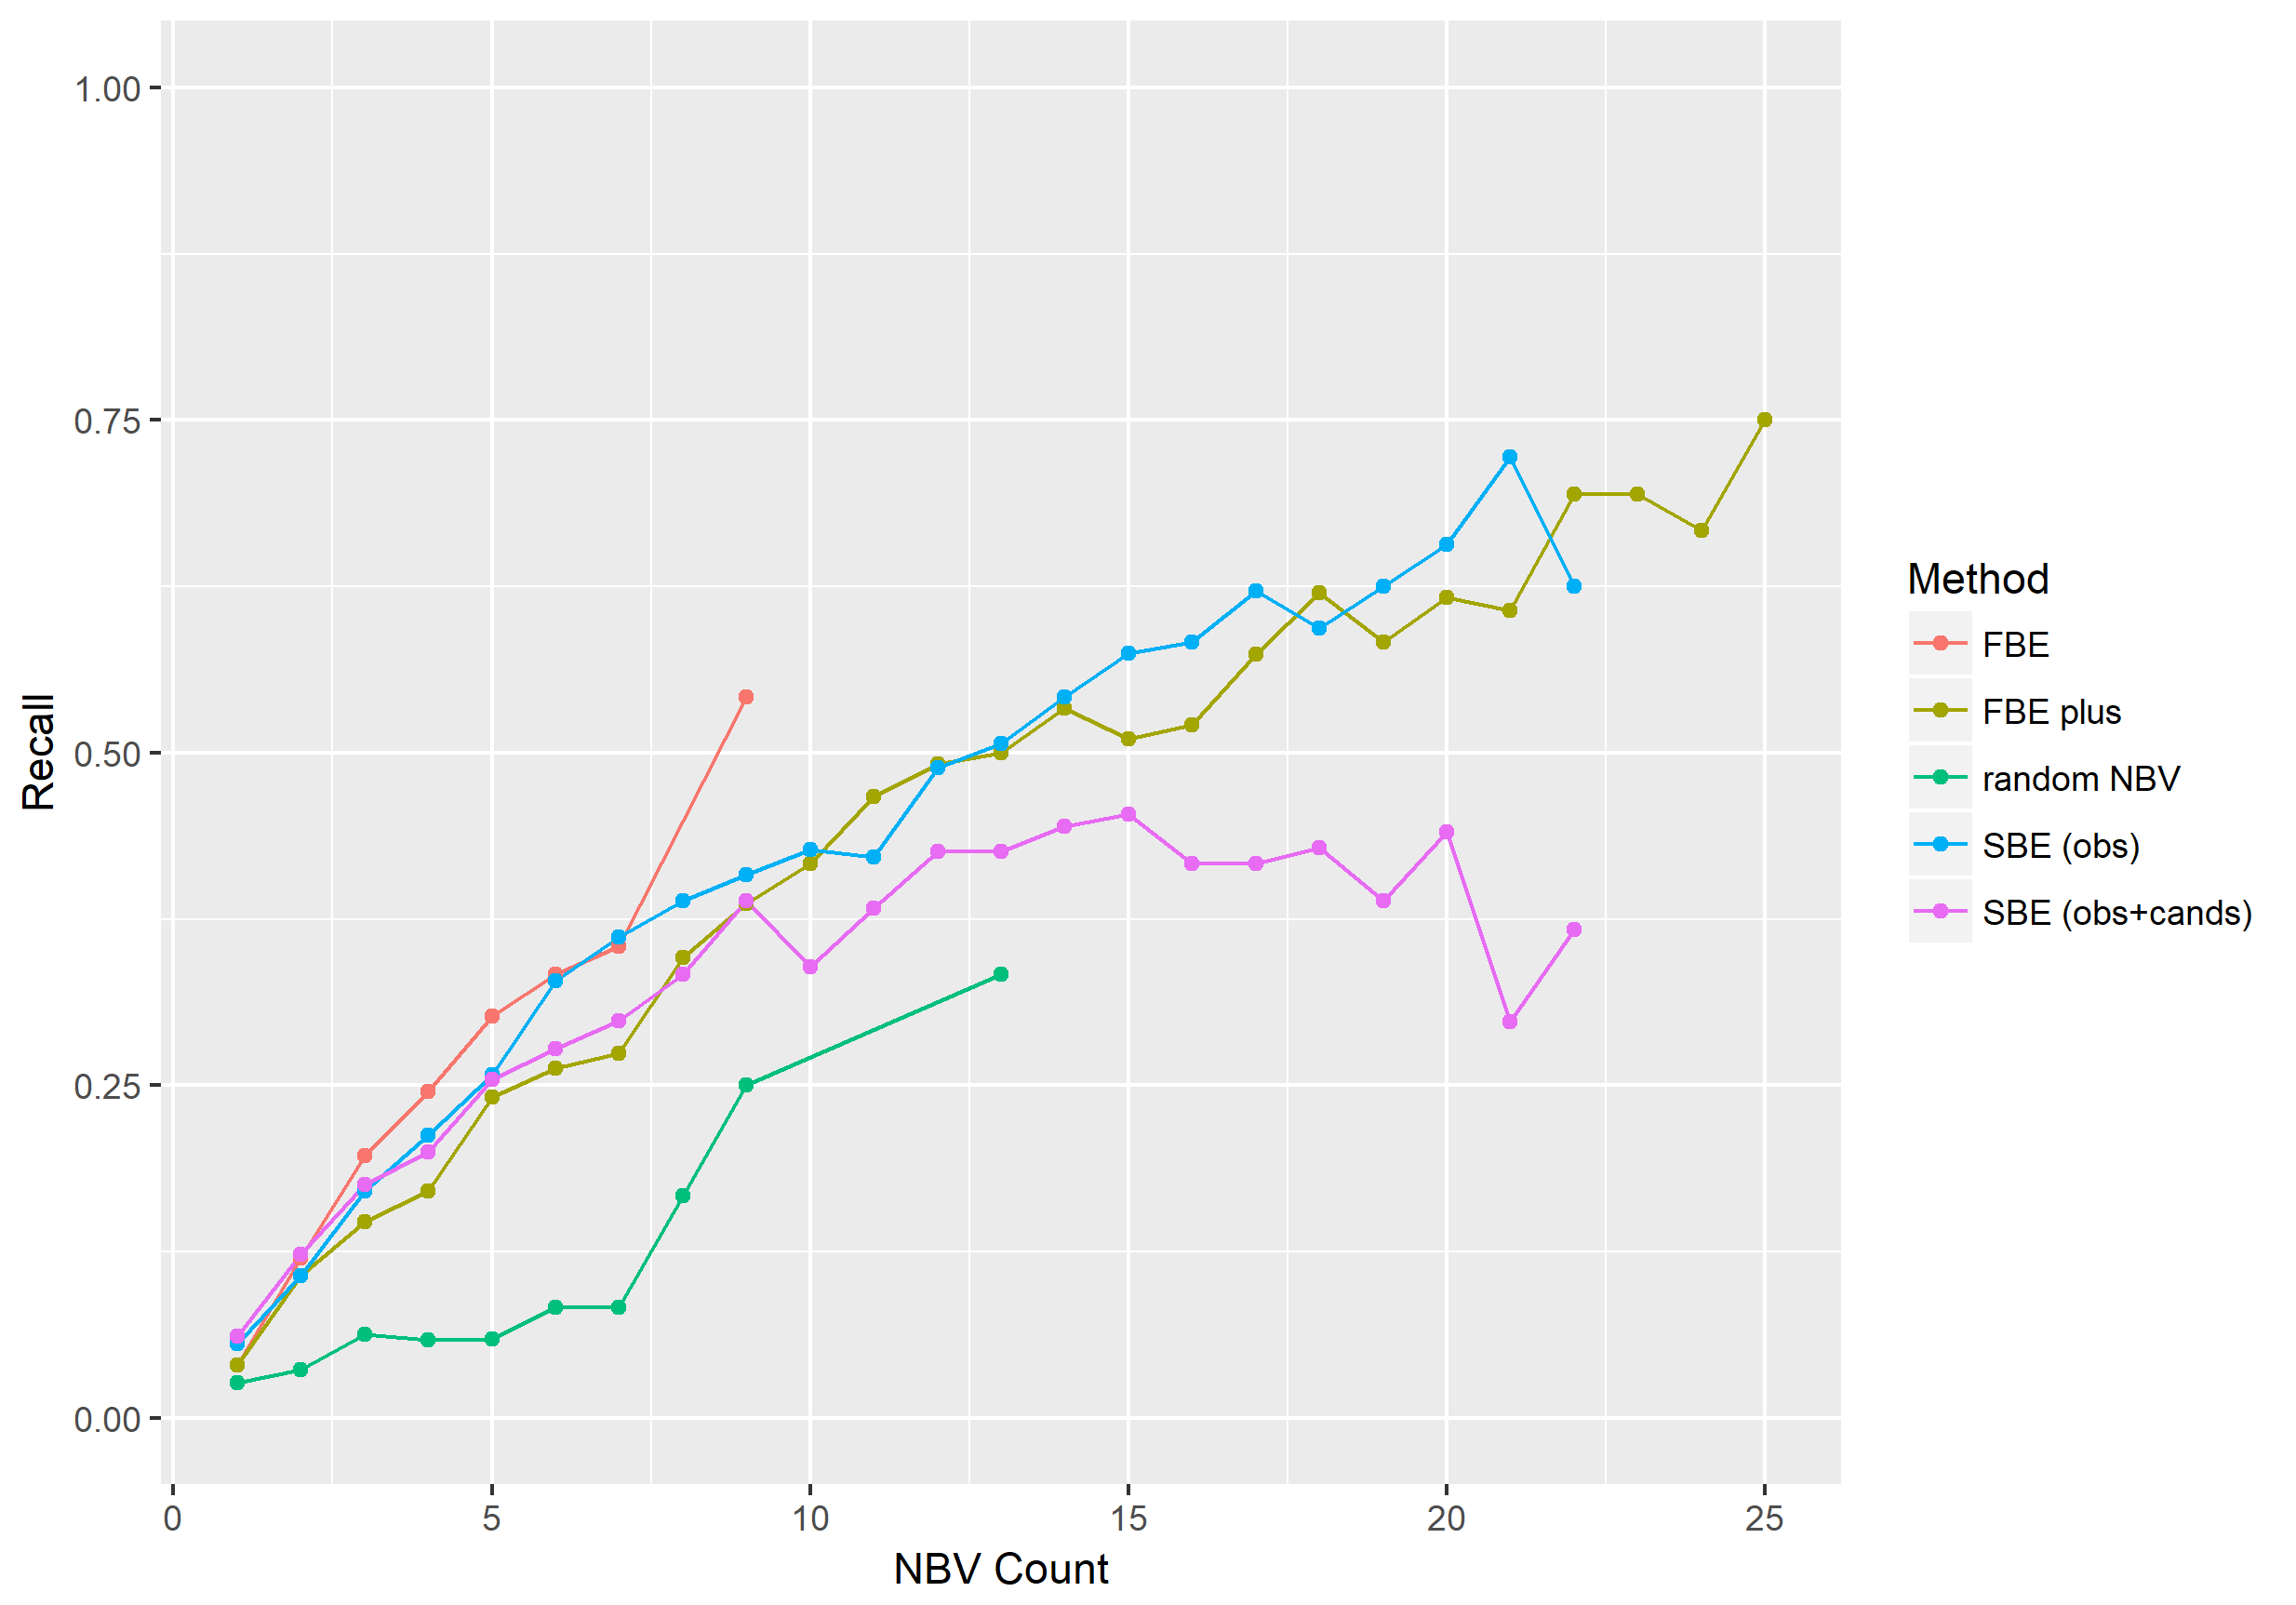
\includegraphics[width=0.8\linewidth]{src/Plots/recall_vs_nbv_count_scattered.png}
			\caption{Development of object-level recall for different NBV methods}
		\end{figure}

		\vspace{0.5cm}
  	
		%----------------------------------------------------------------------------------------
		%	FUTURE WORK
		%----------------------------------------------------------------------------------------

		\begin{block}{Possible extensions}
		
		\large{
				\begin{itemize}
					\item Improve SLAM system
					\item Include depth information in object candidate computation
					\item Use heuristics to estimate the shapes of unseen areas of objects
				\end{itemize}}

		\end{block}

		\vspace{1cm}

		% \begin{center}
		% \begin{tabular}{ccc}
		% \hfill 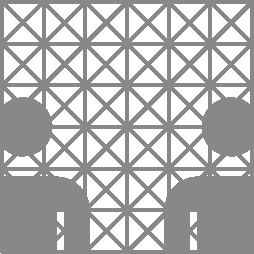
\includegraphics[width=0.2\linewidth]{src/infIcon.pdf} ~ 
\includegraphics[width=0.2\linewidth]{src/uhhIconR.pdf} \hfill
		% \end{tabular}
		% \end{center}

  \end{column}
	
\end{columns}

\end{block}

% \begin{columns}[t,totalwidth=\twocolwid]

% 	\begin{column}{\onecolwid}

% 		%----------------------------------------------------------------------------------------
% 		%	CONCLUSION
% 		%----------------------------------------------------------------------------------------

% 		% \begin{block}{Conclusion}

% 		% Nunc tempus venenatis facilisis. \textbf{Curabitur suscipit} consequat eros non porttitor. Sed a massa dolor, id ornare enim. Fusce quis massa dictum tortor \textbf{tincidunt mattis}. Donec quam est, lobortis quis pretium at, laoreet scelerisque lacus. Nam quis odio enim, in molestie libero. Vivamus cursus mi at \textit{nulla elementum sollicitudin}.

% 		% \end{block}
		
% 	\end{column}	

% 	\begin{column}{\sepwid}\end{column} % Empty spacer column

% 	\begin{column}{\onecolwid}

		
		
% 	\end{column}
	
% \end{columns}

\end{column}


% \begin{column}{\onecolwid}
	
% 	%----------------------------------------------------------------------------------------
% 	%	ADDITIONAL INFORMATION
% 	%----------------------------------------------------------------------------------------

% 	\begin{block}{Additional Information}

% 	Maecenas ultricies feugiat velit non mattis. Fusce tempus arcu id ligula varius dictum. 
% 	\begin{itemize}
% 	\item Curabitur pellentesque dignissim
% 	\item Eu facilisis est tempus quis
% 	\item Duis porta consequat lorem
% 	\end{itemize}

% 	\end{block}

% 	%----------------------------------------------------------------------------------------

% \end{column} % End of the third column

\end{columns} % End of all the columns in the poster

\end{frame} % End of the enclosing frame

\end{document}
